\section{Технологический раздел}
В этом разделе обосновывается выбор средств программной реализации метода.
Будут приведены результаты разработки программного обеспечения, реализующее метод удаления импульсных шумов из цветных изображений.
Будут описан формат входных и выходных данных.
Будут показаны демонстрация работы программы и принципы, применяющиеся в тестировании.
Будут приведены результаты предварительного тестирования разработанного программного комплекса.

\subsection{Средства реализации программного комплекса}
Перед тем, как программно реализовать метод, нужно перечислить требования к средствам реализации программного комплекса:
\begin{enumerate}
	\item Язык программирования должен иметь библиотеки, позволяющие работать со сверточными нейронными сетями а также с большими массивами данных.
	\item Среда разработки должна поддерживать выбранный язык программирования.
	\item Требуется ориентироваться на облачные вычисления, так как они позволяют не использовать локальные вычислительные ресурсы.
\end{enumerate}

В качестве среды разработки был использован проект Yandex DataSphere.
Он позволяет на платной основе использовать облачные вычислительные ресурсы, в частности процессор NVIDIA Tesla V100.

Также в возможности DataSphere входит версионирование моделей и сохранение сеанса сессии, в отличие от аналогов.

\subsubsection{Выбор языка программирования}
Для написания программного обеспечения был использован язык Python.
Это обусловлено следующими причинами:
\begin{itemize}
	\item имеется опыт разработки на данном языке;
	\item для Python было реализовано множество библиотек, позволяющих работать со сверточными нейронными сетями.
\end{itemize}

Для работы с нейронными сетями была выбрана библиотека tensorflow версии 2.12.

Это обусловлено тем, что на текущий момент tensorflow показывает более высокие показатели производительности, чем другие аналоги, например, pytorch.
Также у автора имеется опыт использования данной библиотеки для разработки сверточных нейронных сетей.

В качестве библиотеки для работы с изображениями был выбран OpenCV, так как в ней присутствуют модули, позволяющие взаимодействовать с функциями из tensorflow.

\subsection{Формат входных и выходных данных}
В качестве входного параметра выступают два обязательных параметра:
\begin{enumerate}
	\item Путь до изображения в формате jpg или jpeg размера, большего чем 40 x 40 пикселей.
	\item Тип импульсного шума, который нужно очистить: шум соли или шум перца.
\end{enumerate}

Также пользователь имеет возможность указать путь до базового изображения для расчета метрик качества очистки изображения от шумов.

На выходе метод образует изображение такого же размера, что и исходное изображение, но очищенное от шумов.
Если пользователь задал базовое изображение без шумов, то программа также рассчитывает и метрики качества очистки изображений.

\subsection{Реализация программного комплекса}
Реализация программного комплекса делится на три основные части: реализация и обучение нейронной сети, реализация модуля взаимодействия с пользователем и реализация модуля обработки изображений. 
В комплекс действий также входит и создание собственного датасета для обучения модели, так как текущие датасеты содержат либо исходные изображения без шумов, либо искаженные гауссовым шумом.
Также требуется реализовать алгоритмы, использующиеся в самом методе.

\subsubsection{Нейронная сеть}
Исходную базу изображений, требуемых для обучения модели, потребовалось разбить на небольшие изображения размером 40 × 40 пикселей, так как это предусмотрено в модели. 
Код алгоритма разбиения модели на пачти представлен на листинге \ref{lst::patch} (приложение А).

Для увеличения набора тестовых данных некоторые изображения подвергались предварительным преобразованиям, таким как поворот и обрезка.
Общий алгоритм сбора данных для обучения нейросети представлен на листинге \ref{lst::dataset} (приложение А).

Конфигурация всех нейронных сетей основана на методе RIDNET, но количество модулей EAM было уменьшено до трех в целях уменьшения времени, потраченного на обучения моделей.
При этом в качестве функции активации используется сигмоида, что позволило улучшить точность результатов, однако увеличило время обучения сети.
Реализация структуры представлена на листинге \ref{lst::neuron} (приложение А).

Модель использовала адаптивную оценку момента в качестве функции оптимизации.
Метод требует вычисление экспоненциального скользящего среднего градиента и квадратичный градиент.

Реализация обучения нейронной сети представлена на листинге \ref{lst::train} (приложение А).

\subsubsection{Результаты обучения нейронной сети}
Обучение производилось с помощью процессора NVIDIA Tesla V100.
Объем оперативной памяти машины составлял 392 ГБ, на видеопамять выделялось 32 ГБ памяти.
Это позволило ускорить процесс обучения: одна эпоха занимала 51 секунду, в то время как на процессоре Inter Core i5 аналогичный процесс длился около 2 часов.
Каждая из моделей прошла обучение в 20 эпох для достижения результата.

По результатам обучения модель выделила суммарно 1515731 параметров. 
В процессе обучения модель выдает два параметра после каждой эпохи:
\begin{itemize}
	\item loss -- значение функции потерь для обучающей выборки, с учетом того, что некоторые нейроны отбрасывались из обучения во время эпохи;
	\item val\_loss -- значение функции потерь для обучающей выборки, но нейросеть использует все нейроны.
\end{itemize}

График для метрики loss представлен на рисунке \ref{tech::loss}:
\FloatBarrier
\begin{figure}[h]	
	\begin{center}
		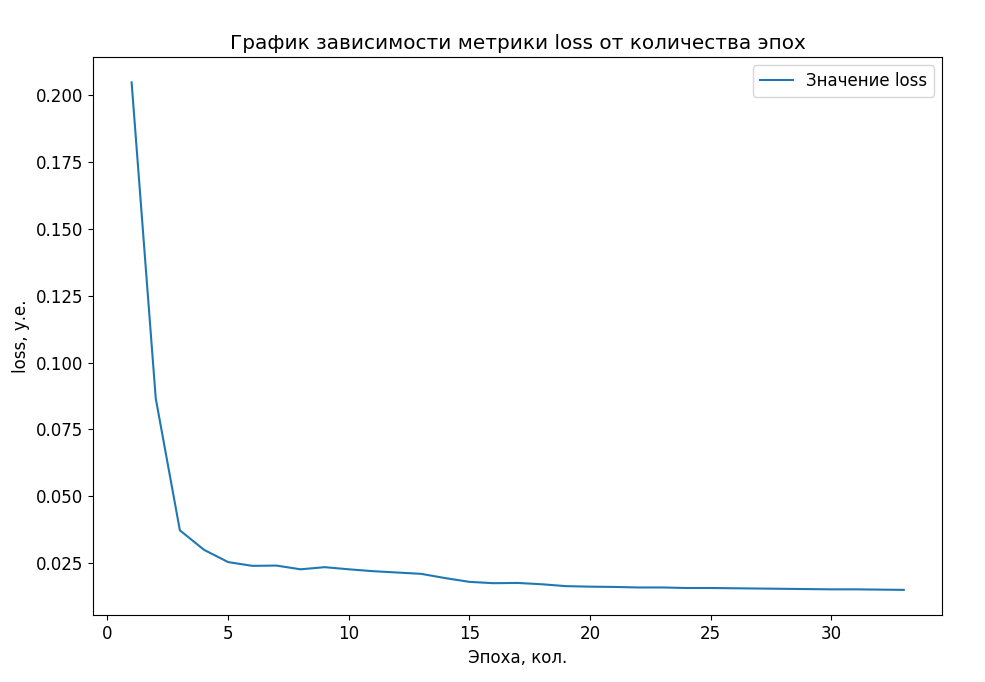
\includegraphics[width=\linewidth]{inc/png/loss.png}
	\end{center}
	\captionsetup{justification=centering}
	\caption{График зависимости loss от эпохи}
	\label{tech::loss}
\end{figure}
\FloatBarrier

По графику можно сделать следующие выводы:
\begin{itemize}
	\item график имеет вид гиперболы;
	\item уже к 5 эпохе значение loss составляет 0.025, в дальнейшем значение меняется слабо, соответственно, в случае недостатка вычислительных ресурсов пяти эпох уже достаточно для достижения результата.
\end{itemize}

\newpage
График для метрики val\_loss представлен на рисунке \ref{tech::val_loss}:
\FloatBarrier
\begin{figure}[h]	
	\begin{center}
		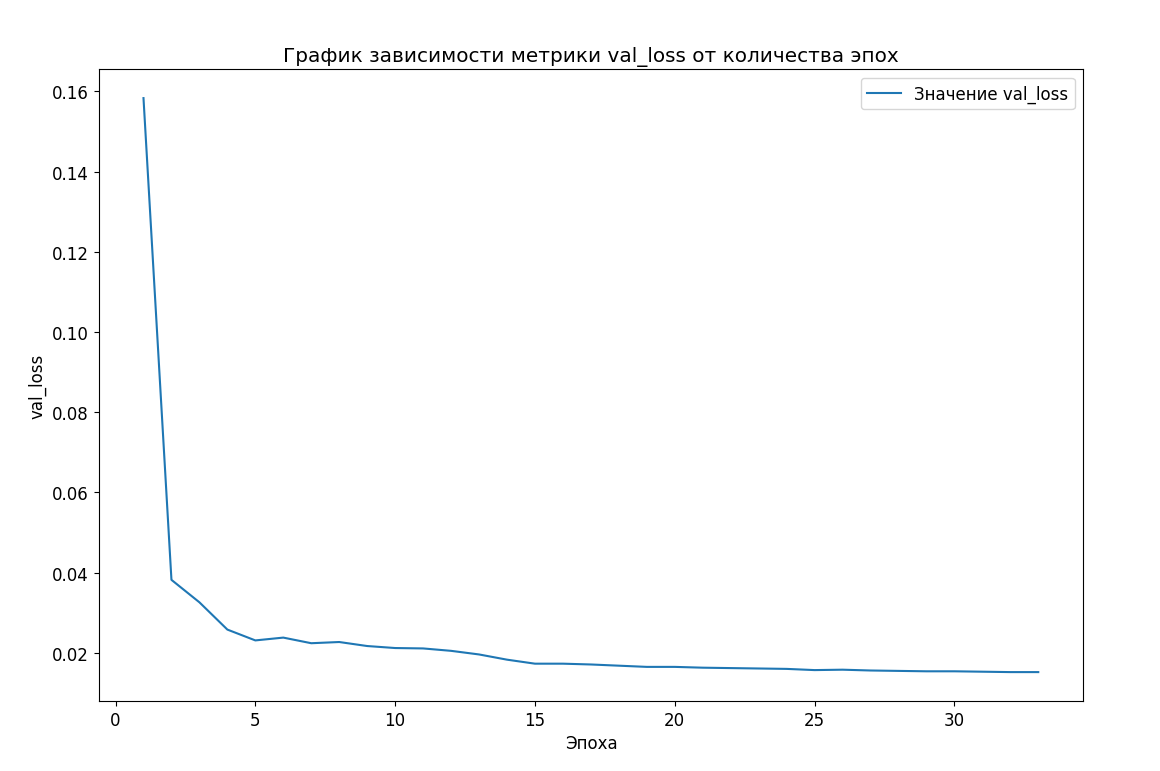
\includegraphics[width=\linewidth]{inc/png/val_loss.png}
	\end{center}
	\captionsetup{justification=centering}
	\caption{График зависимости loss от эпохи}
	\label{tech::val_loss}
\end{figure}
\FloatBarrier

Значение метрики val\_loss меньше, чем значение loss по состояние на ту же эпоху. 
График также имеет вид гиперболы, но до 15 эпохи график изменяется как дробно-линейная функция.
Для достижения приемлемого результата также оказалось достаточно 5 эпох. 
Последние эпохи также не оказывают влияния на итоговые метрики модели.

Исходя из этого, можно сделать вывод, что в случае ограниченности вычислительных ресурсов достаточно обучить нейронную сеть на пяти эпохах. 
Для достижения результата будет достаточно 15-20 эпох, так как в дальнейшем функция потерь перестает изменяться.

\subsubsection{Реализация метода}
Для реализации метода требовались обученные нейронные сети, реализация которых приведена в предыдущем разделе.

Также требовалась реализация алгоритма, позволяющего оценить количество шума на патче.
Реализация представлена на листинге \ref{lst::shum}:
\FloatBarrier
\begin{lstinputlisting}
	[language=Python, caption=Реализация алгоритма оценки количества шума, linerange = {62-70},
	basicstyle=\footnotesize\ttfamily, label={lst::shum}, frame=single, breaklines=true]{inc/src/clean\_module.py}
\end{lstinputlisting}
\FloatBarrier

Реализация общего алгоритма работы представлена на листинге \ref{lst::common} (приложение Б).

Также для применимости медианного фильтра и нейронной сети для восстановления изображения нужно было провести некоторые преобразования.
Исходное изображение представлено массивом из библиотеки numpy, в то время как нейронная сеть использует другое представление пикселей.
Реализация алгоритма приведена на листинге \ref{lst::median}:
\FloatBarrier
\begin{lstinputlisting}
	[language=Python, caption=Реализация медианного фильтра, linerange = {48-59},
	basicstyle=\footnotesize\ttfamily, label={lst::median}, frame=single, breaklines=true]{inc/src/clean\_module.py}
\end{lstinputlisting}
\FloatBarrier

После применения всех алгоритмов к патчам требуется восстановить изображение.
Код функции, выполняющий реставрацию полученного изображения из кусков представлен на листинге \ref{lst::heal} (приложение Б).

\newpage
\subsection{Демонстрация работы программы}
В результате разработки был программно реализован метод, позволяющий удалить шумы из изображения.

Стартовый экран для пользователя представлен на рисунке \ref{tech::start}:
\FloatBarrier
\begin{figure}[h]	
	\begin{center}
		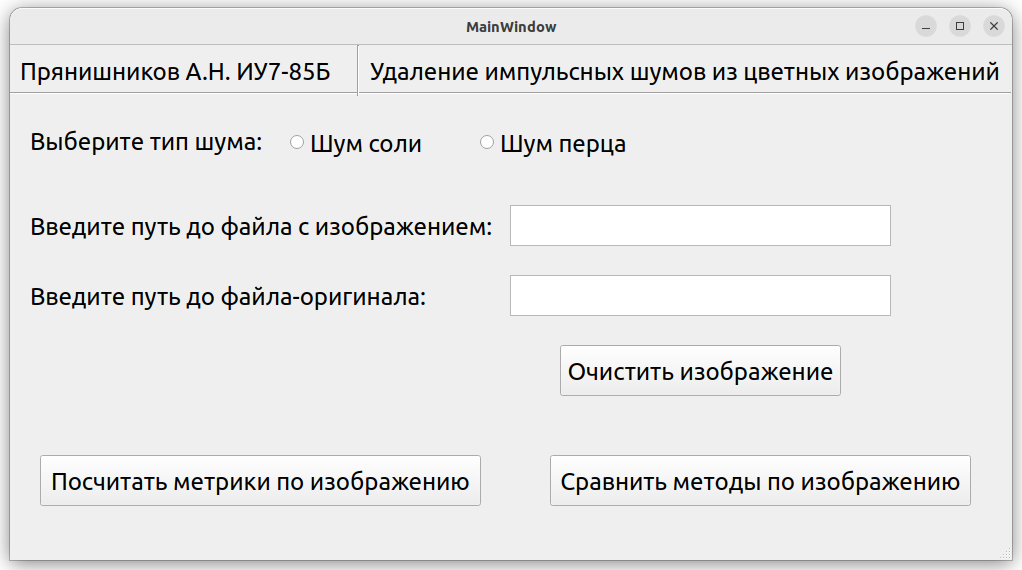
\includegraphics[width=\linewidth]{inc/png/startUI.png}
	\end{center}
	\captionsetup{justification=centering}
	\caption{Стартовый экран}
	\label{tech::start}
\end{figure}
\FloatBarrier

Пользователю доступны следующие возможности:
\begin{enumerate}
	\item Очистка изображений от шумов. Для этого нужно выбрать тип шума и ввести путь до загрязненного изображения.
	\item Посмотреть значение метрики PSNR для конкретного изображения. Для этого нужно помимо параметров для очистки требуется указать путь до оригинального изображения.
	\item Сравнить с другими методами. В этом случае не требуется вводить дополнительные данные. Программа построит график сравнения эффективности методов на заранее заданном датасете.
\end{enumerate}

\newpage
Пример работы по очистке изображений представлен на рисунке \ref{tech::res}:
\FloatBarrier
\begin{figure}[h]	
	\begin{center}
		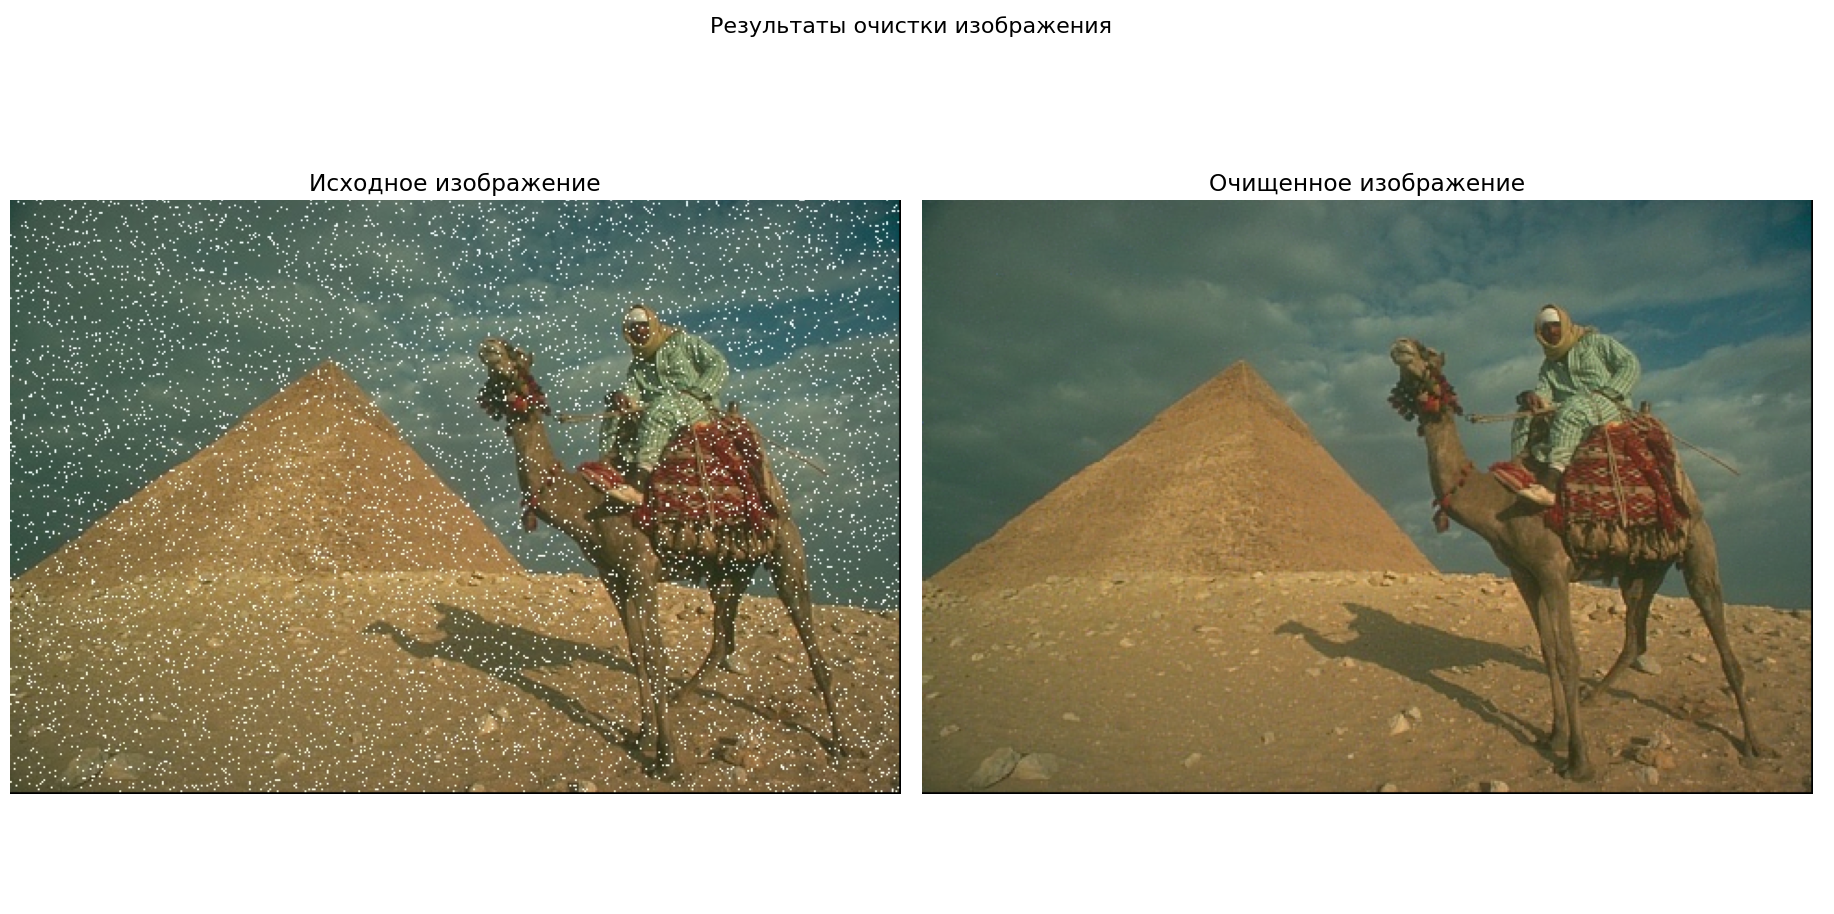
\includegraphics[width=\linewidth]{inc/png/result2.png}
	\end{center}
	\captionsetup{justification=centering}
	\caption{Пример работы программы}
	\label{tech::res}
\end{figure}
\FloatBarrier

\subsection{Тестирование разработанного метода} 
Для тестирования метода были сформулированы следующие требования:
\begin{enumerate}
	\item Тестирование происходит на тестовой выборке, загрязненной шумами нужного типа.
	Процент шума при этом между изображениями отличается.
	\item Зашумленность изображения не превышает 30\%. Этого достаточно для оценки корректности работы модели.
	\item Модель должна давать по каждому изображению значение метрик большее, чем у исходного загрязненного изображения.
\end{enumerate}

Тестирование проводилось на исходном датасете, но в изображения был добавлен синтетический шум.
Среднее значение по каждому проценту шума усреднялось, но шум соли и перца учитывался как один вид шума.

\newpage
Результаты по загрязненности шума были визуализированы с помощью графика, который представлен на рисунке \ref{tech::test}:
\FloatBarrier
\begin{figure}[h]	
	\begin{center}
		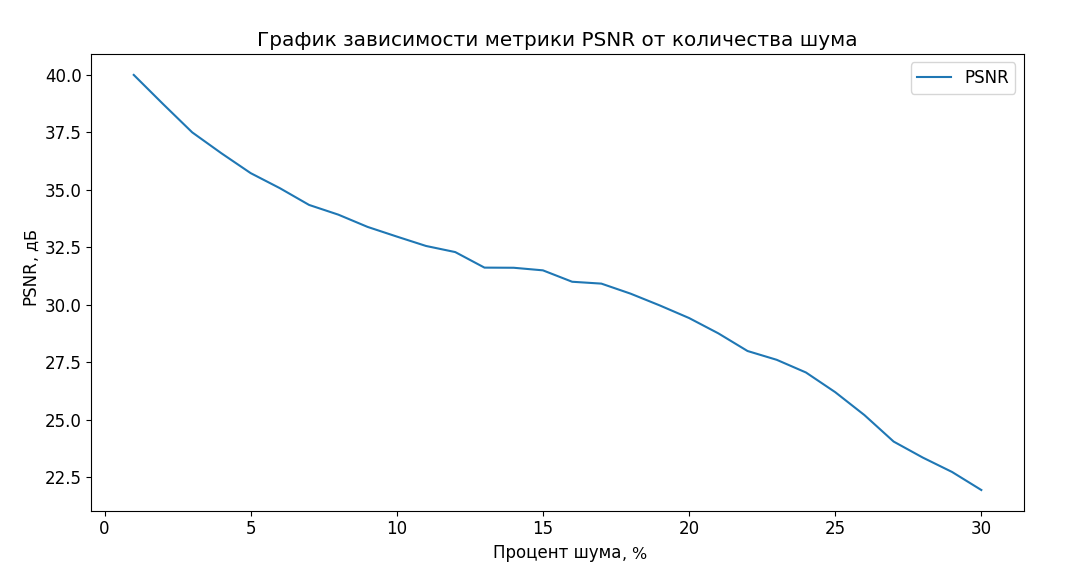
\includegraphics[width=\linewidth]{inc/png/testing1.png}
	\end{center}
	\captionsetup{justification=centering}
	\caption{Результаты тестирования разработанного метода}
	\label{tech::test}
\end{figure}
\FloatBarrier

Видно, что метрики эффективности метода уменьшаются с ростом количества шумов, но результат соответствует поставленным требованиям.

\subsection*{Выводы}
Был обоснован выбор средств программной реализации методы.
Был реализован метод, позволяющий удалить импульсные шумы из цветных изображений.
Было показано, что для обучения нейронной сети достаточно пяти эпох, чтобы достичь заметного результата, приведен график зависимости метрик нейронной сети от эпох.

Было создано приложение с графическим интерфейсом, позволяющее применить метод на практике и оценить его эффективность.
Было проведено тестирование, которое показало, что метод является работоспособным на изображениях.